\pdfoutput=1

\documentclass[11pt]{article}
\usepackage[UTF8]{ctex}


\usepackage[final]{acl}

\usepackage{times}
\usepackage{latexsym}
\usepackage{xcolor}
\usepackage{tcolorbox}

\usepackage{tabularx}
\usepackage{booktabs}
\usepackage{enumitem}
\usepackage[T1]{fontenc}

\usepackage[utf8]{inputenc}

\usepackage{microtype}
\usepackage{amsmath}
\usepackage{amssymb}
\usepackage{colortbl}
\usepackage{booktabs}
\usepackage{pifont}
\usepackage{xcolor}
\usepackage{multirow}
\usepackage{inconsolata}

\usepackage{graphicx}
\definecolor{darkgreen}{rgb}{0.0, 0.5, 0.0}
\newcommand{\greencheck}{\textcolor{darkgreen}{\ding{51}}}

\hypersetup{
    colorlinks=true,
    linkcolor=red,
    citecolor=cyan,
    filecolor=magenta,
    urlcolor=cyan,
    }

\title{
MedCoT:通过分层专家的医学思维链
}

\author{
 \textbf{Jiaxiang Liu\textsuperscript{1}}\ \ \
 \textbf{Yuan Wang\textsuperscript{1}}\ \ \
 \textbf{Jiawei Du\textsuperscript{2, 3}}\ \ \
 \textbf{Joey Tianyi Zhou\textsuperscript{2, 3}}\ \ \
 \textbf{Zuozhu Liu\textsuperscript{*, 1}}
\\
\\
 \textsuperscript{1} \small ZJU-Angelalign R\&D Center for Intelligence Healthcare, Zhejiang University, China\\
 \textsuperscript{2} \small Centre for Frontier AI Research (CFAR), Agency for Science, Technology and Research (A*STAR), Singapore
\\
 \textsuperscript{3} \small Institute of High Performance Computing (IHPC), Agency for Science, Technology and Research (A*STAR), Singapore
\\
 { \small
   {\tt \{jiaxiang.21, zuozhuliu\}@intl.zju.edu.cn}
 }
}
\begin{document}

\maketitle

\begin{abstract}
人工智能在医学视觉问答 (Med-VQA) 领域取得了进展,但普遍的研究往往侧重于答案的准确性,而忽略了推理路径和可解释性,这在临床环境中至关重要。此外,目前的 Med-VQA 算法通常依赖单一模型,缺乏实际医疗诊断所需的稳健性,而这些诊断通常需要专家的协作评估。
为了解决这些不足,本文提出了 MedCoT,一种新颖的分层专家验证推理链方法,用于增强生物医学成像查询的可解释性和准确性。MedCoT 基于两个原则:\textit{Med-VQA 中明确推理路径的必要性}和\textit{制定准确结论所需的多专家审查}。该方法涉及初步专家提出诊断理由,然后由跟进专家验证这些理由,最后通过本地部署的诊断专家中的稀疏专家混合进行投票达成共识,从而提供最终诊断。
在四个标准 Med-VQA 数据集上的实验评估表明,MedCoT 超越了现有的最先进方法,在性能和可解释性上提供了显著的提升。
代码发布于 \url{https://github.com/JXLiu-AI/MedCoT}。
\let\thefootnote\relax\footnotetext{* 责任作者。}
\end{abstract}
\section{引言}

\begin{figure}[t!]
\centering
\includegraphics[width=0.45\textwidth]{image/Figure_1_v7.pdf}
\caption{
上图显示了先前 Med-VQA 方法与 MedCoT 的输出比较,以及 MMCoT 中的先前技术 \cite{zhang2023multimodal} 与 MedCoT 中的稀疏 MoE 的比较。
下图展示了 MedCoT 模型规模约为 256M 参数,在 VQA-RAD 和 SLAKE-EN 数据集上的准确率分别超越 7B 参数的 LLaVA-Med 5.52\% 和 4.09\%。
}
\label{fig1}
\end{figure}

医学视觉问答(Med-VQA)最近引起了广泛关注 \cite{chen2022align, gong2021cross, ren2020cgmvqa, khare2021mmbert}。作为医学领域的新探索,Med-VQA旨在基于输入的医学图像回答自然语言的医学问题。一个有效的Med-VQA系统可以帮助临床医生解释医学图像,从而确保和加速诊断过程。对于患者来说,自动化的Med-VQA服务可以极大地满足个性化健康咨询的需求 \cite{liu2023parameter}。

在Med-VQA领域,已经有许多基于深度学习技术的尝试 \cite{tiong2022plug, banerjee2020weaqa, changpinyo2022all, liu2023chatgpt, gai2024medthink}。例如,\citet{nguyen2019overcoming} 使用双线性注意网络(BAN)\cite{kim2018bilinear},并通过结合预训练元学习模块和卷积去噪自编码器(CDAE)组成的混合增强视觉特征(MEVF)设置对其进行了增强。基于此,\citet{zhan2020medical} 设计了一个条件推理框架,以提升Med-VQA模型的推理能力。然而,这些方法在许多实际场景中往往表现不佳,主要是因为在从有限数量的医学图像和文本数据中提取和整合特征方面能力不足 \cite{eslami2021does, song2022clip, wang2022clip}。
\citet{eslami2021does} 引入了CLIP架构,将其作为MEVF中的视觉编码器 \cite{nguyen2019overcoming},并在多模态医学数据集ROCO上进行预训练 \cite{pelka2018radiology}。他们的实验表明,CLIP显著提高了性能。\citet{liu2023parameter} 开发了VQA-Adapter,使用轻量级适配器和标签平滑技术高效微调CLIP模型用于Med-VQA,从而降低了计算成本并减轻了过拟合。
\citet{li2024llava} 提出了LLaVA-Med,利用GPT-4和一种新的课程学习方法高效训练LLaVA在生物医学图像上的表现,显著增强了Med-VQA的能力。

然而,以往的Med-VQA方法通常关注于答案的准确性 \cite{nguyen2019overcoming,liu2023parameter,zhan2020medical},其中大多数MedVQA响应只包含简单的答案,缺乏详细的解释或推理,不同于现实世界中医生不仅提供答案,还解释其推理、专业考虑和可能的矛盾,以得出更全面的诊断见解。
此外,现实世界的诊断往往依赖于多位医生的综合经验,因为单一医生的诊断可能会受到个人经验的偏见,可能不够准确。
在多模态思维链(CoT)中,回答VQA问题涉及提供答案以及相应的推理路径(理由)。
这种理由的生成有助于提高语言模型的准确性。
受现实世界实践和多模态CoT \citet{zhang2023multimodal,zheng2023ddcot} 的启发,将这种范式整合到Med-VQA中可以增强答案的准确性和可解释性。然而,实施它面临几个挑战:(1)以前的CoT方法需要手动标注基本理由,这既耗时又昂贵,且难以保证一致性和完整性 \cite{zhang2023multimodal,zheng2023ddcot}。(2)依赖单一专家模型可能导致误导性结论。(3)多模态CoT在理解图像和文本意图的深度上有限,这可能限制其在医学背景下的有效性 \cite{zhang2023multimodal}。

为了解决上述问题,我们引入了MedCoT,一种分层的专家验证模型用于Med-VQA。首先,初始专家根据医学视觉和文本查询提出初步诊断理由。随后,后续专家审核这些理由,将其分类为有效或无效;有效的理由被保留,而无效的则需要重新评估。
最后,局部实现的诊断专家,由一个稀疏专家混合(MoE)模型组成,作为多模态语言模型进行投票,以提供明确的诊断。
通过利用层级化的专业知识,MedCoT在四个大型数据集上持续优于最先进的(SoTA)Med-VQA方法,展示了令人印象深刻的泛化能力和可解释性,如\autoref{fig1}所示。
我们的研究做出了三个重要贡献:

\begin{itemize}
    \item 我们对在多模态CoT中生成推理的挑战和见解进行了深入分析。我们的研究结果表明,单一专家往往无法提供明确的验证,在处理关于特定器官的问题时更容易出错。
    \item 受现实世界诊断的启发,我们开发了不需要手动标注推理的分层专家验证MedCoT。这涉及三个层次的专家验证:初始、跟进和诊断。MedCoT不仅提供更准确的答案,还提供更精细的推理。
    \item 在诊断阶段,我们设计了包含多数投票的稀疏MoE。该框架的多个专业专家能够高效且准确地解释医学图像和文本的意图,使诊断专家能够提供精确的回应。

\end{itemize}

\vspace{1em}

\begin{figure*}
\centering
\includegraphics[width=\textwidth]{image/Figure_pipeline_v7.pdf}
\caption{ MedCoT 流程首先由初始专家接收医疗问题和图像,以生成初步推理。该推理可能存在缺陷(用红色标记),随后由后续专家进行审查。如果推理被认为有效,则保留;否则,将重新考虑,并生成新的推理(用绿色标记),以及图像说明。然后将这些元素整合到诊断专家中。在所有背景信息的指导下,诊断专家作为一种设计了稀疏 MoE 结构的多模态语言模型,给出最终诊断结果(答案)。 }
\label{MedCoT pipeline}
\vspace{-1em}
\end{figure*}
\section{相关工作}
\vspace{-0.5em}
\subsection{Med-VQA}
VQA 是计算机视觉和自然语言处理中的一种多模态任务,旨在用自然语言对图像的查询进行响应 \cite{ben2019vqa,he2020pathvqa,ren2020cgmvqa}。它涉及特征提取、融合和推理,以理解多模态意图并管理特征处理。Med-VQA 将 VQA 扩展到医学领域,在此领域中,强大的医学知识对于回答特定领域的问题至关重要 \cite{liu2023parameter},这使得特征提取更加复杂。Nguyen 等人的创新如 MEVF 利用无监督的 CDAE 和元学习来初始化专门针对 Med-VQA 的权重 \cite{nguyen2019overcoming}。Zhan 等人基于此开发了一种条件推理框架来处理不同类型的问题 \cite{zhan2020medical},而 Eslami 等人成功地将 CLIP 模型作为视觉编码器实施,证明了其在该背景下的有效性 \cite{eslami-etal-2023-pubmedclip}。LLaVA-Med 利用 GPT-4 和一种新颖的课程学习方法对生物医学图像进行训练 \citet{li2024llava},显著增强了 Med-VQA 的能力。虽然能够进行互动对话,但其回答并不注重通向答案的推理路径。MedCoT 不同于上述方法,它不仅提供精确的答案,还提供推理路径(理由)。此外,其有效性通过分层专家验证得到确认,更加符合现实世界的医疗场景。
\subsection{多模态链式推理}
使用大型语言模型(LLMs)的链式推理(CoT)在自然语言处理方面已显示出成功。多模态链式推理将视觉信息与传统的文本链式推理相结合,整合综合数据以执行推理任务 \cite{zhang2023multimodal,zheng2023ddcot}。在多模态链式推理的开创性工作 \cite{zheng2023ddcot,zhang2023multimodal,lu2022learn,lu2023chameleon,zhang2023llama} 中,首先在ScienceQA数据集上进行研究。ScienceQA包括多模态科学问题及带注释的推理 \cite{lu2022learn}。MM-CoT开发了一个基于ScienceQA的两阶段框架,训练模型从注释中生成推理,随后用于形成最终答案 \cite{lu2022learn}。 随着开放世界知识在LLMs中越来越多的整合,研究正致力于为这些模型配备视觉模态,以应对复杂的视觉和多模态挑战。例如,DDCoT \cite{zheng2023ddcot} 引入了角色特定的链式推理,将问题分解为子问题,并使用LLMs重新组合原则,提高精度并在多模态环境中解决语言错觉。 受到这些进展的启发,我们旨在将多模态链式推理适用于医学领域,以提高Med-VQA的可解释性和准确性。
\subsection{MoE}
MoE通过结合多个专家网络并使用门控网络根据给定输入确定哪些专家被激活来优化学习和预测 \cite{zhang2024scalable,fedus2022switch}。稀疏MoE是MoE模型的一种变体,在每次预测中仅激活少数专家,从而有效利用计算资源并增强可扩展性 \cite{shazeer2016outrageously}。
稀疏MoE模型在计算机视觉和自然语言处理领域的条件计算背景下被独立探索 \citet{jacobs1991adaptive,fedus2022review}。条件计算旨在增加模型参数的数量而不成比例地增加计算成本。这是通过根据输入特定因素有选择地激活模型的相关部分来实现的 \cite{shazeer2016outrageously}。稀疏MoE模型采用一种学习的门控机制,仅为给定输入激活一部分专家,特别是从\( N \)个专家中选择\( k \)个。这允许选择所有专家或仅选择稀疏组合,从而优化资源使用 \citet{lepikhin2020gshard}。

\begin{figure}[t]
\centering
\includegraphics[width=0.5\textwidth]{image/Figure_3_v7.pdf}
\caption{诊断专家流程。 医学图像通过视觉编码器后生成视觉特征。 包括图像标题、推理过程和选项在内的上下文文本信息通过文本编码器处理,以获取文本特征。 然后通过交叉注意进行特征整合,产生组合特征。 这些整合特征与文本特征一起输入到稀疏 MoE 结构中。 在这里,多个专业专家深入理解图像和文本的意图。 然后将这些理解输入到文本解码器中,解码信息以产生最终答案。 }
\label{Diagnostic}
\vspace{-1em}
\end{figure}
\section{方法论}
\subsection{预备知识}
在整篇论文中,我们将 Med-VQA 任务建模为一个多模态 CoT 框架,如下所示:该框架以图像 \( I \) 和问题 \( Q \) 作为输入,并输出推理依据 \( R \)。这个推理依据 \( R \) 随后用于生成答案 \( A \)。这种范式确保了过程的透明性,提供了从输入到结论的可追溯路径,这对于验证结果和提高用户对框架诊断能力的信任至关重要。我们可以将 Med-VQA 任务建模为一个多模态 CoT,如下所示:
\begin{equation}
    \min_{f, g} \mathbb{E}_{(I, Q, A^*) \sim \text{Data}} \left[ L \left( g \left( f(I, Q), I, Q \right), A^* \right) \right].
\end{equation}

函数 \( f \) 负责生成合理且有帮助的推理依据 \( R \)(初始和后续专家),而函数 \( g \) 使用这个推理依据生成最终答案 \( A \)(诊断专家)。推理依据 \( R \) 来源于初始专家的评估和后续专家的自我反思。最终答案 \( A \) 由诊断专家通过损失函数 \( L \) 确定,该损失函数衡量预测答案 \( A \) 与真实答案 \( A^* \) 之间的差异。
\subsection{初始专家}
在初始诊断阶段,我们指示 LLMs 作为主要推理诊断专家。
我们向 LLMs 提示以下指令:
\textit{"请进行逐步分析并提供理由"} ($prompt_{\hat{i}}$)。
这样做是为了指导 LLMs 执行详细的、逐步的推理过程。
从中获得的文本理由表示为 \( R_{\hat{i}} = LLMs(T, I, prompt_{\hat{i}}) \),其中 \( T \) 和 \( I \) 分别表示文本和图像输入。\( T \) 包括问题 \( Q \) 和选项等文本上下文。
\( prompt_{\hat{i}} \) 是用于引出理由的特定提示策略。有关提示的更多技术细节,请参阅附录。

例如,如\autoref{MedCoT pipeline}所示,对于问题 "Is there a localized mass?",我们获得了一个高度可解释的理由(用于最终诊断结果):"The provided chest X-ray image shows bilateral interstitial infiltrates, which could indicate the presence of a localized mass"。
\subsection{后续专家}
在后续诊断阶段,我们指导LLMs进行自我反思推理,并在问题的背景下进行测试,以识别有效的推理,保留它们,并重构无效的推理以生成准确的推理。具体来说,我们通过以下提示来引导LLMs:
\textit{"请判断这个推理对问题和图像是否有效。如果有效...,如果现有推理无效..."} ($prompt_{\hat{f}}$)。完整的提示内容请参见附录。我们可以使用以下公式定义后续专家的自我反思推理:
\begin{equation}
\begin{small}
R_{\hat{f}} =
\begin{cases}
R_{\hat{i}} & \text{if } R_{\hat{i}} = \text{Effective} \\
\text{LLMs}(T, I, {prompt}_{\hat{f}}) & \text{if } R_{\hat{i}} = \text{Ineffective},
\end{cases}
\end{small}
\end{equation}
其中 $R_{\hat{f}}$ 是后续专家的推理。此过程帮助我们获得诊断分析所需的文本推理,如\autoref{MedCoT pipeline}所示。

为了为诊断专家注入更多知识并弥合图像和文本之间的差距,我们利用后续专家生成图像说明。此过程有助于减少模态差距,有效地将这些知识传递给诊断专家。有关详细的图像说明提示,请参见附录。
\subsection{诊断专家}
我们使用基于多模态T5结合稀疏MoE的设计模型来作为诊断专家,如 \autoref{Diagnostic} 所示。诊断专家接收丰富的文本上下文和医学影像信息,以生成最终的诊断结果。
\subsubsection{多模态 T5}

\autoref{Diagnostic} 显示了多模态 T5 的结构,包括 \textit{TextualEncoder}、\textit{VisualEncoder}、\textit{Cross-Attention Network}、稀疏 MoE 和 \textit{TextualDecoder}。以下是网络的详细信息:

\textit{TextualEncoder} 将自然语言输入 \( {T} \) 转换为文本特征空间 \( F_T \in \mathbb{R}^{n \times d} \),而 \textit{VisualEncoder} 将输入图像 \( I \) 转换为视觉特征 \( F_I \in \mathbb{R}^{m \times d} \)。
这里,\( n \) 表示输入语言文本的长度,\( d \) 表示隐藏特征的维度,\( m \) 表示图像块的数量。
在获得文本表示 \( F_T \) 和视觉表示 \( F_I \) 后,我们的模型利用 \textit{Cross-Attention Network} 进行模态交互。该网络计算注意力引导的视觉特征 \( H_{V}^{\text{att}} \in \mathbb{R}^{n \times d} \),它选择性地捕获响应文本查询的相关视觉特征,如下操作所示:
\begin{align}
        H_{V}^{\text{att}} &= \text{Softmax}\left(\frac{QK^{\top}}{\sqrt{d}}\right)V,
\end{align}
其中 $Q$, $K$, $V$ 分别从 $F_T$, $F_I$, $F_I$ 中导出,分别对应查询、键和值。

一旦获得注意力引导的视觉特征 \( H_{V}^{\text{att}} \) 和文本表示 \( F_T \),我们构建 MoE 动态地将它们结合,得到 \( F_F = \text{MoE} (H_{V}^{\text{att}}, F_T) \)。MoE 的详细信息将在以下章节提供。
$F_{\text{ F}}$ 被输入到 \textit{TextualDecoder} 中以生成答案
$A = \text{TextualDecoder}(F_{\text{F}})$,如 \autoref{Diagnostic} 所示。

在训练中,改进使预测答案 (A) 更准确地逼近标签答案。具体而言,输入模型 $f$ 最大化正确序列 $Y = {A}$ 的似然。损失函数 $L$ 是所有标记的负对数似然,给出为:$L = -\sum_{n=1}^{N} \log p(Y_n | X, Y_1^{n-1})$,其中 $N$ 是标记的数量,$p(Y_n | X, Y_1^{n-1})$ 是预测 $Y$ 中正确的第 $n$ 个标记的概率。
\subsubsection{MoE}

在多模态CoT中,一个关键步骤是理解图像和文本的意图并做出相应的响应。
然而,以前的方法主要使用门控来进行整合,其中门控函数 \( \lambda = \text{Sigmoid}(W_l F_T + W_v H_V^{\text{att}}) \) 权重衡量图像相对于源文本的重要性,\( W_l \) 和 \( W_v \) 是可学习的参数(见附录)\cite{zhang2023multimodal, zheng2023ddcot}。
根据我们的实验结果显示,门控是不够的(\autoref{ablation})。
因此,MedCoT 提出了构建一个 MoE 用于整合过程。

稀疏 MoE 实现了一个 top-k 的稀疏专家混合 \cite{fedus2022switch},利用多个稀疏专家专门处理复杂的 Med-VQA 数据。
该模块根据门控得分动态选择每个输入的 top-k 专家,如 \autoref{Diagnostic} 所示。

在获得专家的输出后,我们使用特征级多数投票来聚合它们的输出。
每个专家的权重使用下列公式计算:
\begin{align}
    \text{W}_i = \text{softmax}(\text{V}^{\text{top k}})_i = \frac{e^{\text{V}^{\text{top k}}_i}}{\sum_{j=1}^{k} e^{\text{V}^{\text{top k}}_j}},
\end{align}

其中 \(\text{W}_i\) 是第 \(i\) 个被选中专家的权重,\(\text{V}^{\text{top k}}_i\) 是第 \(i\) 个被选中专家的得分。
对于每个特征 \( F_f \),特征级多数投票的最终结果通过加权平均所有选定专家的输出来计算:
\begin{align}
    {E}_{F_f} = \sum_{i=1}^{k} \text{W}_i \cdot E_{i, F_f} ,
\end{align}
其中 \({E}_{F_f}\) 是特征 \( F_f \) 的最终结果值,\(E_{i, F_f}\) 是第 \(i\) 个选中专家对特征 \( F_f \) 的输出。然后,
\(\lambda = \text{Sigmoid}({E}_{F_f}) \)。
最终,这导致 \( F_f \) 结果如下:
\begin{align}
    F_{\text{F}} &= (1-\lambda) \cdot F_{\text{T}} + \lambda \cdot H_{V}^{\text{att}}.
\end{align}

稀疏 MoE 网络允许每个选定专家处理他们擅长的数据,如 \autoref{rad} 所示,展示了擅长解决头部相关问题的专家。

\begin{figure}[t]
\centering
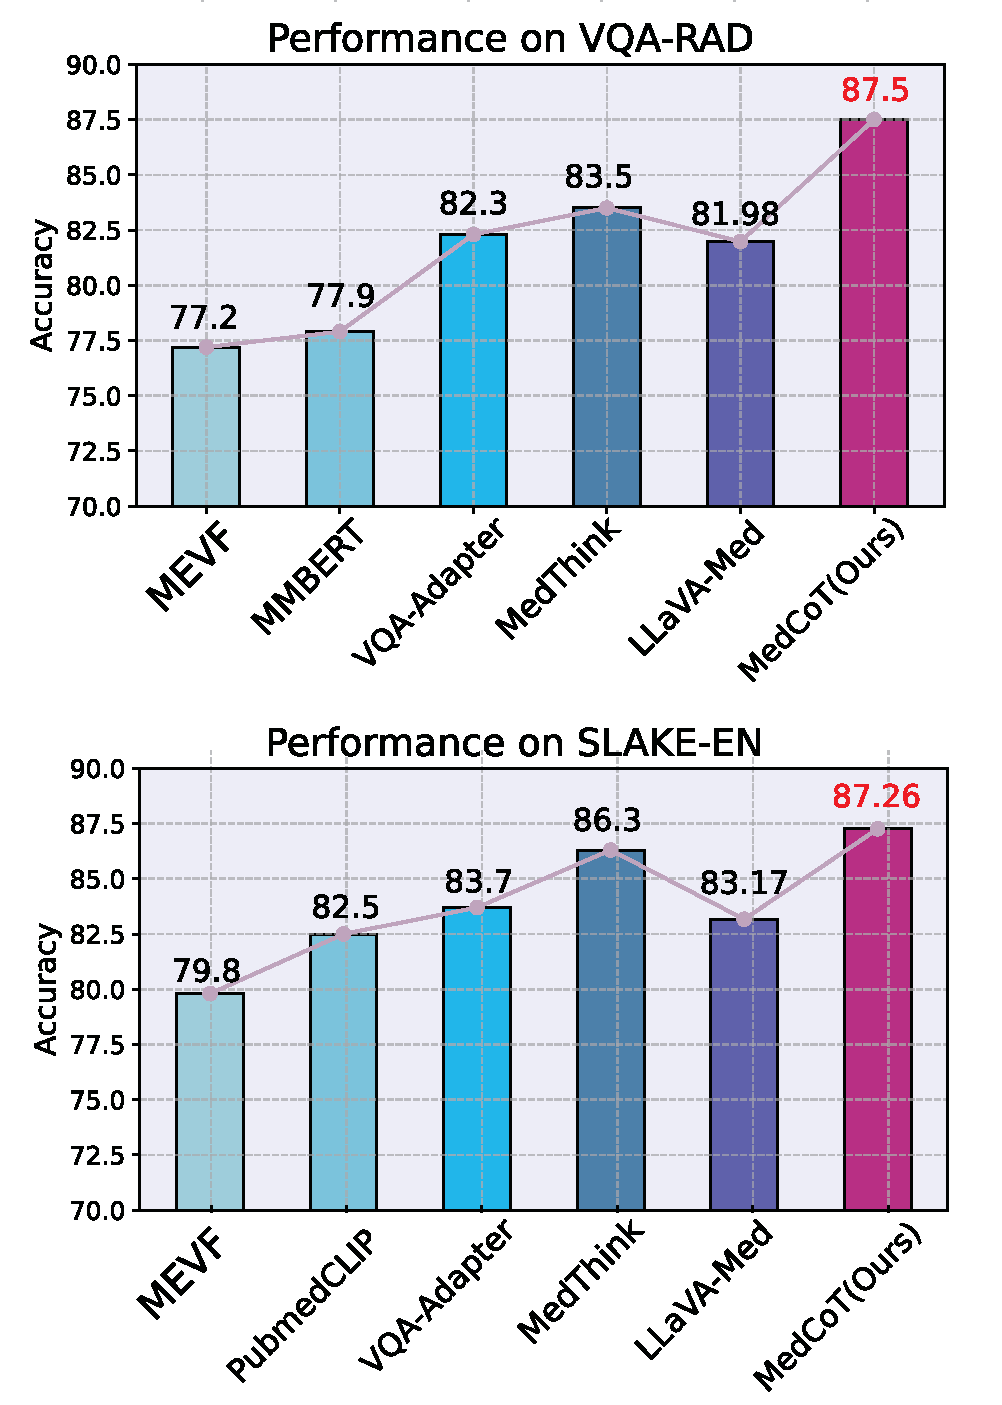
\includegraphics[width=0.4\textwidth]{image/Performance5.pdf}
\caption{
MedCoT 与多种 SoTA 方法在 VQA-RAD 和 SLAKE-EN 数据集的封闭问题上进行比较。 MedCoT 不仅在答案上达到 SoTA 准确率,还提供推理路径(理由)。 使用的指标是准确率(\%)。
}
\label{performance}
\vspace{-1em}
\end{figure}

\begin{figure*}
\centering
\includegraphics[width=\textwidth]{image/Figure_case1_v3.pdf}
\caption{
MedCoT 管道从初始专家接收医疗问题和图像开始,以生成初步推理。该推理可能存在缺陷(用红色表示),随后由跟进专家进行审查。如果推理被认为有效,则保留;否则,将重新考虑并生成新的推理(用绿色表示),以及图像说明。这些元素随后会被整合到诊断专家中。在所有背景信息的指导下,诊断专家作为一个具有设计稀疏 MoE 结构的多模态语言模型,提供最终的诊断结果(答案)。
}
\label{case1}
\end{figure*}
\section{实验}
\subsection{实验设置}
在MedCoT框架中,Flan-T5 \cite{khashabi2020unifiedqa,raffel2020exploring}的编码器和解码器分别被集成为TextualEncoder($\cdot$)和TextualDecoder($\cdot$)。此外,DETR \cite{carion2020end}被用作VisualEncoder($\cdot$)。
我们的诊断专家模型经过100个epoch的训练,学习率为$8e-5$,批量大小为8。
为了展示MedCoT的效果,我们在医学VQA领域使用了四个基准数据集进行验证:VQA-RAD \cite{lau2018dataset},SLAKE-EN \cite{liu2021slake},Med-VQA-2019 \cite{abacha2019vqa},和PathVQA \cite{he2020pathvqa}。详细统计信息见附录。
所有实验都是使用PyTorch \cite{paszke2019pytorch}和HuggingFace \cite{wolf2020transformers}进行的,具体实现是在4个NVIDIA GEFORCE RTX 3090 GPU上完成的。准确率被用作评估指标。
对于LLMs,我们的初步专家和后续专家使用Gemini Pro 1.5版本。更多的实验细节可以在附录中找到。

\begin{figure}
\centering
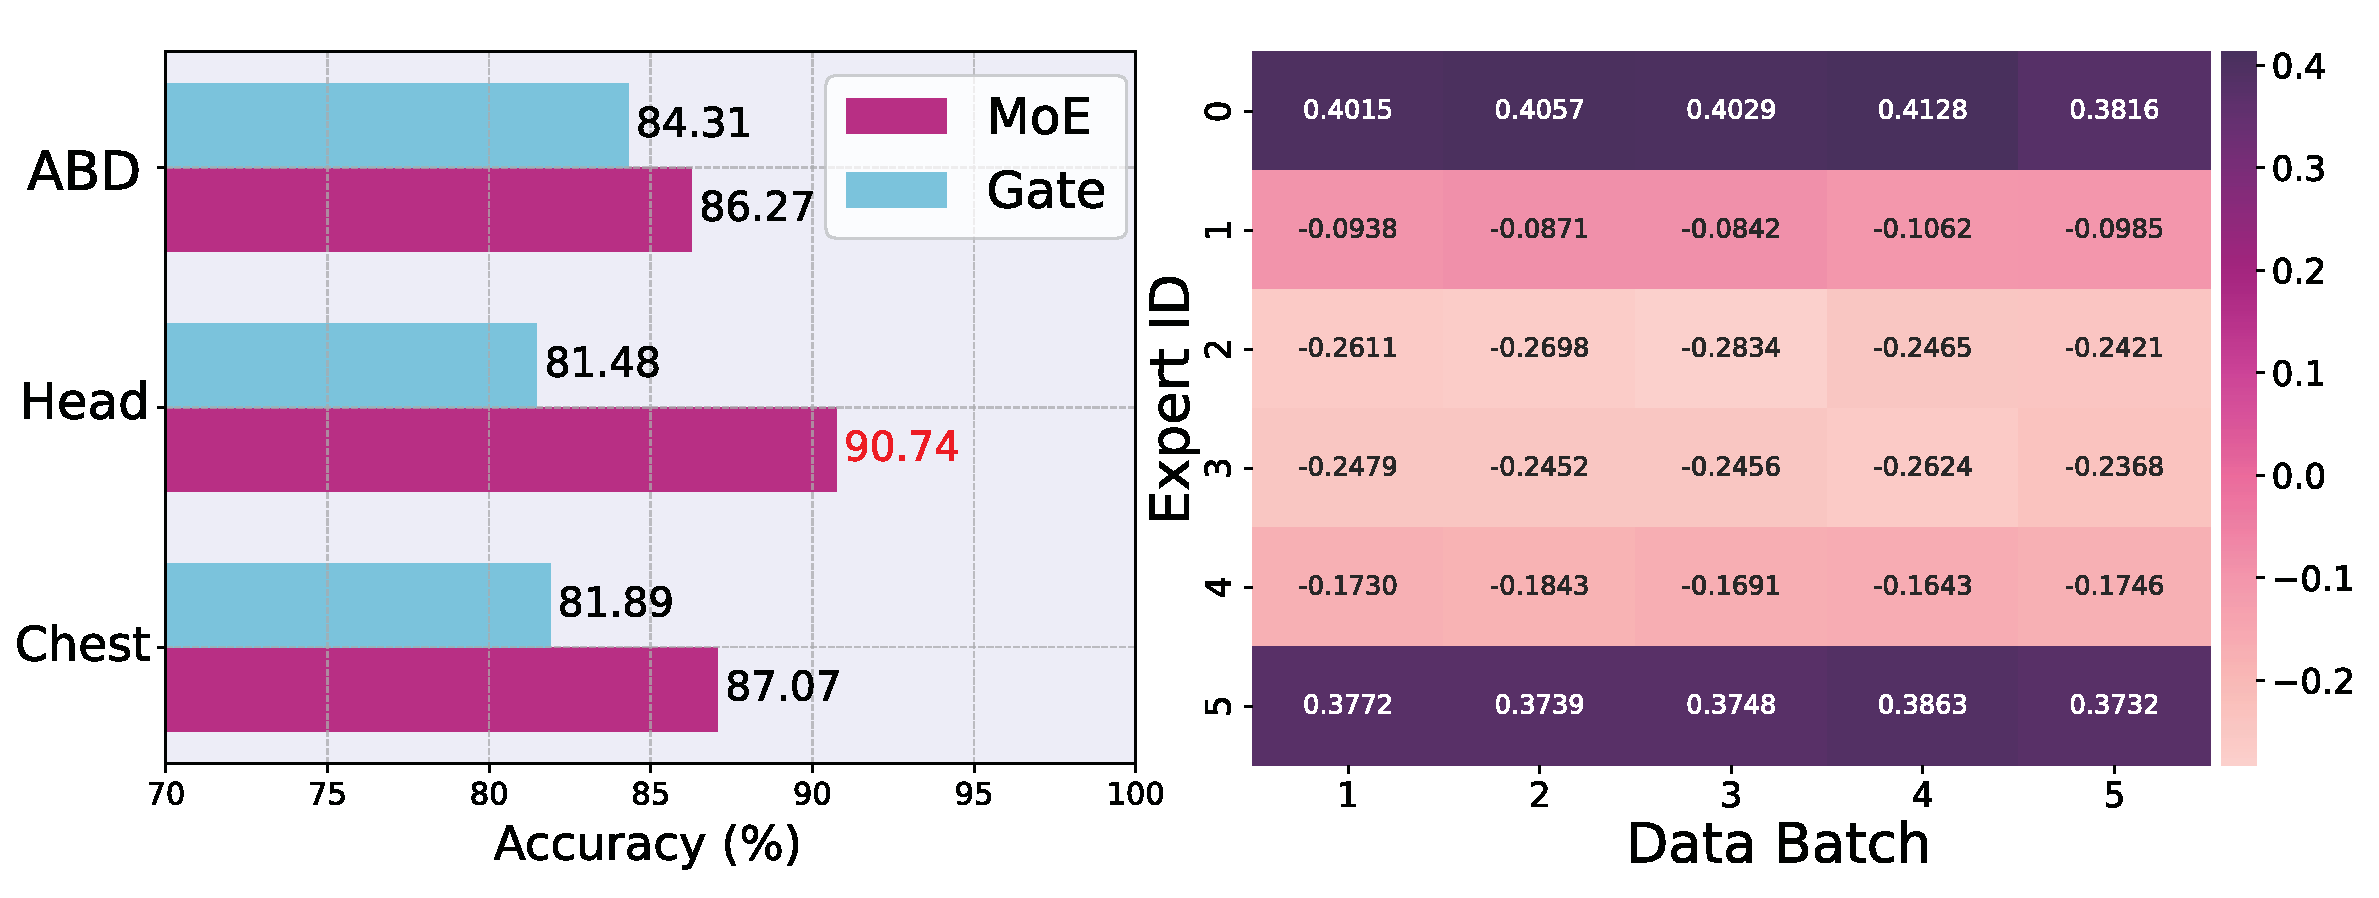
\includegraphics[width=0.5\textwidth]{image/RAD-v4.pdf}
\caption{
诊断专家的稀疏 MoE 在 VQA-RAD 中对不同器官相关问题显示出不同的准确性水平。
'ABD' 代表腹部相关问题,'Head' 指头部相关问题,'Chest' 指胸部相关问题。
可以观察到头部相关问题的准确率提高了近 10 \%。我们可视化了专家的权重(右图)。值得注意的是,在前 2 个专家选择中,模型选择了专家 0 和专家 5 来理解“头部”图像和文本的意图。
}
\label{rad}
\end{figure}

\begin{figure*}
\centering
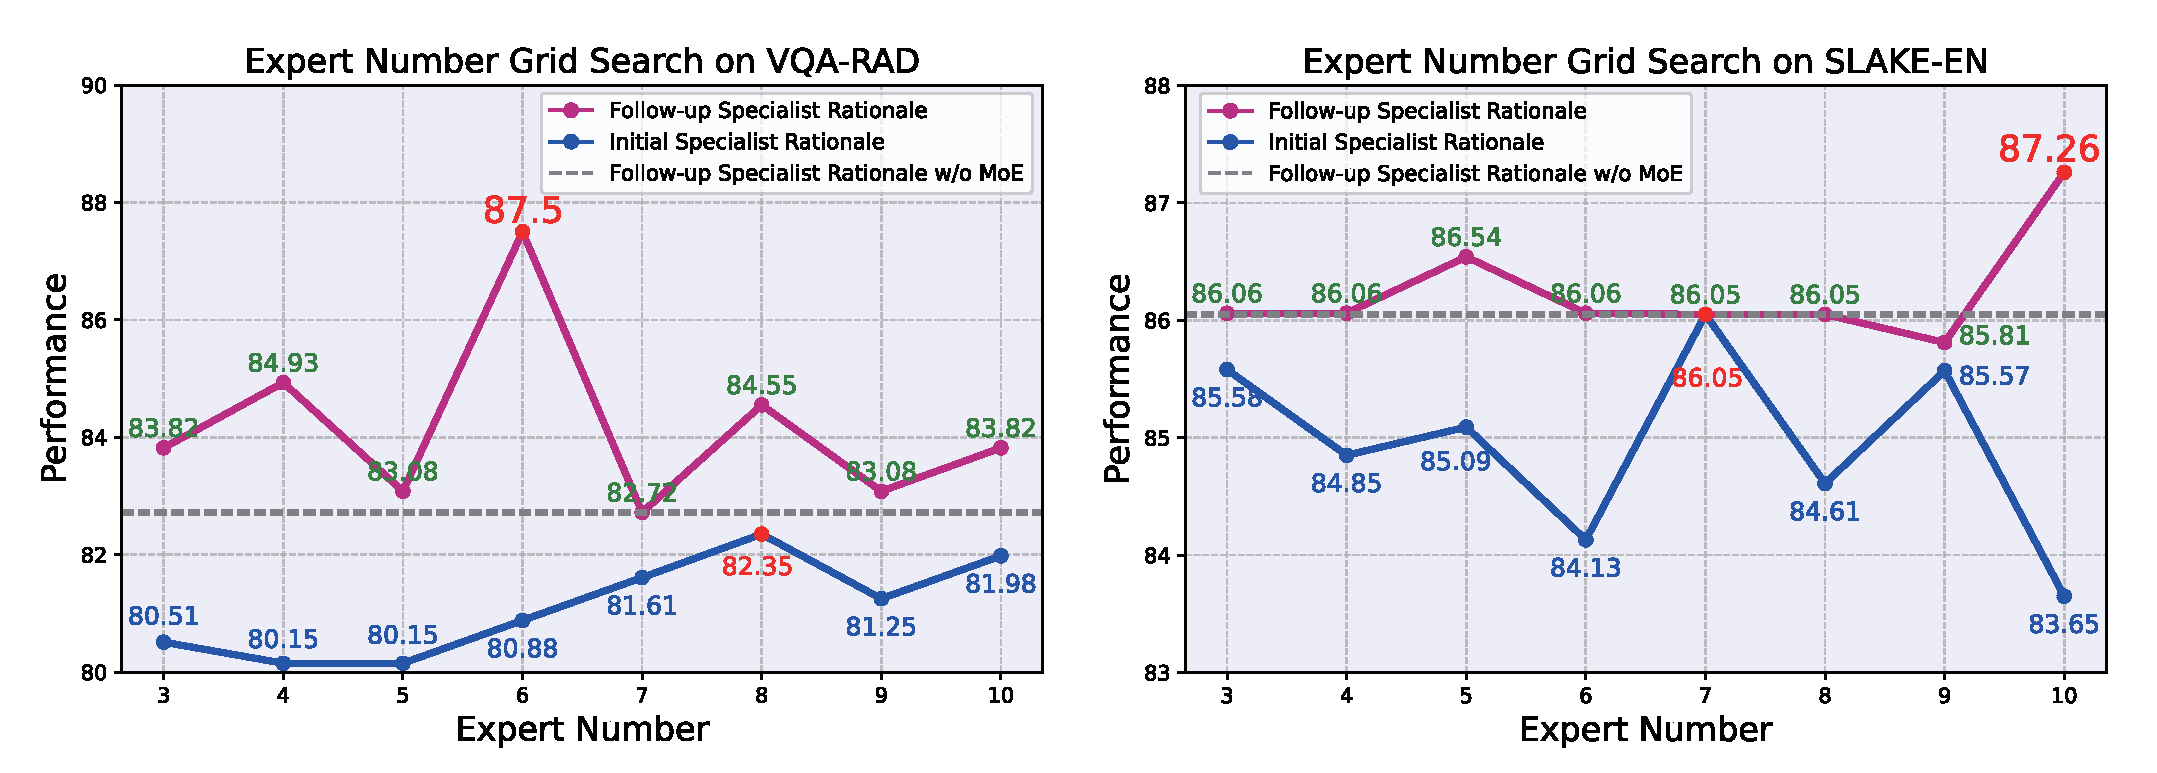
\includegraphics[width=0.9\textwidth]{image/zhexiantu_all_v6.pdf}
\caption{在两个数据集上的专家数量网格搜索。蓝线表示使用初始专家推理进行训练以及在诊断专家中进行专家数量网格搜索的结果。紫线表示使用后续专家推理并进行专家数量网格搜索的结果。灰线表示诊断专家在没有稀疏 MoE 情况下使用后续专家推理的结果。}
\label{zhexiantu-all}
\vspace{-1em}
\end{figure*}
\subsection{主要结果}
我们在 VQA-RAD 和 SLAKE-EN 数据集上评估 MedCoT 的性能,并与 MEVF \cite{nguyen2019overcoming}、MMBERT \cite{tiong-etal-2022-plug}、PubMedCLIP \cite{eslami-etal-2023-pubmedclip}、VQA-Adapter \cite{liu2023parameter}、MedThink \cite{gai2024medthink}、LLaVA-Med \cite{li2024llava} 等已建立的模型进行基准测试。

我们的性能评估分为两个部分,分别关注封闭式问题和开放式问题。封闭式问题结构为单项选择题,使用准确率作为性能指标进行评估,如 \autoref{performance} 所示。面对封闭式问题,MedCoT 在 VQA-RAD 和 SLAKE-EN 数据集上超越了一系列 SoTA 方法。值得注意的是,MedCoT 在这两个数据集上分别比 Gemini 提高了 27.21\% 和 14.66\%,表明单一模型的不可靠性。此外,MedCoT 的微调参数大小约为 256M,优于经过大量医学数据训练的 7B 参数 LLaVA-Med,在两个数据集上分别超过了 5.52\% 和 4.09\%。此外,与之前的方法相比,MedCoT 清晰地展示了推理路径(理由),如 \autoref{MedCoT pipeline} 所示。更多的比较方法结果可以在附录中看到。

相比之下,开放式问题由于其固有的特性允许多种答案。MedCoT 生成的答案很难与数据集精确匹配。因此,我们使用文本生成指标,如 Rouge 和 BLEU 来评估 MedCoT 的性能。我们在开放式 VQA-RAD 和 SLAKE-EN 上进行了实验,结果见附录。MedCoT 在 VQA-RAD 和 SLAKE-EN 数据集上显示出更高的 Rouge 和 BLEU 得分,超越了 MedThink \cite{gai2024medthink}。此外,MedCoT 在 SLAKE-EN 上也显示出更高的得分。

另外,我们还评估了 MedCoT 在 Med-VQA-2019 和 PathVQA 数据集上的性能,如附录所示。结果表明,MedCoT 相较于大多数 SoTA 方法始终实现 SoTA 结果。

\begin{table}
\centering
\small
\setlength{\extrarowheight}{0pt}
\addtolength{\extrarowheight}{\aboverulesep}
\addtolength{\extrarowheight}{\belowrulesep}
\setlength{\aboverulesep}{0pt}
\setlength{\belowrulesep}{0pt}
\caption{关于 MedCoT 的消融研究}
\label{xiaorong}
\begin{tabular}{cc|cc}
\toprule
Follow-up & MoE & VQA-RAD                                        & SLAKE-EN                                        \\
\hline
          &     & 77.57                                          & 83.17                                           \\
   \greencheck       &     & 82.72                                          & 86.05                                           \\
          &  \greencheck   & 80.88                                          & 83.65                                           \\
  \greencheck        &  \greencheck   & {\cellcolor[rgb]{1,0.875,0.757}}\textbf{87.50} & {\cellcolor[rgb]{1,0.875,0.757}}\textbf{87.26}  \\
\bottomrule
\end{tabular}
\end{table}
\subsection{消融研究}
\label{ablation}
\noindent\textbf{后续专家的效果}
为了验证后续专家的有效性,我们将仅包含初始和诊断专家的实验结果与完整的MedCoT进行了对比。正如在\autoref{xiaorong}中所示,在两个医学数据集上,当移除后续专家时,性能显著下降。例如,在VQA-RAD数据集中,性能从87.50\%下降到80.88\%,下降了6.62\%。这证明了后续专家的有效性。

此外,我们进行了仅包含初始和诊断专家的实验,绕过了后续专家的自我反思。在所有涉及不同数量专家的情况下,没有自我反思的结果始终低于经过后续专家反思优化的理由,甚至低于经过自我反思但缺乏MoE组件的诊断专家的结果,如\autoref{zhexiantu-all}所示。这强调了后续专家提供的自我反思的重要性。此外,我们还进行了使用初始和后续专家的零样本实验。正如附录中所示,这些结果进一步确认了后续专家的有效性。

\noindent\textbf{MoE的效果}
为了验证MoE的有效性,我们比较了有无MoE的性能。正如\autoref{xiaorong}中所示,所有数据集中没有MoE时性能显著下降。例如,在VQA-RAD中,性能从87.50\%下降到82.72\%,损失了4.78\%。这表明MoE在诊断专家中起着关键作用。从\autoref{zhexiantu-all}中也可以看出,在大多数专家数量的场景中,缺乏MoE的性能弱于配备稀疏MoE的MedCoT。

此外,我们对VQA-RAD和SLAKE-EN中与器官相关的问题类别进行了实验,如\autoref{rad}所示。显然,在大多数器官相关的问题中,使用MoE的方法优于使用门控机制的方法。值得注意的是,门控机制类似于单专家系统,它在处理头部相关问题时往往表现不佳。在VQA-RAD中的此类问题中,使用MoE的方法比使用门控的方法高出10\%,进一步强调了MoE的有效性。我们可视化了MoE的权重,如\autoref{rad}(右图)所示,显示专家0和5主要处理头部相关问题。这表明这两个专家比门控更有效地动态处理和理解医学图像和文本的意图。在SLAKE-EN上的实验中也可以观察到类似的结果,如附录中所示。

\noindent\textbf{网格搜索}
我们对稀疏MoE中的超参数进行了参数搜索实验,如专家数量和\( k \)值。结果如附录中所示。实验表明,不同数据集的最佳专家数量是不同的。具体而言,VQA-RAD、SLAKE-EN、Med-2019和PathVQA的最佳专家数量分别为6、10、5和5。对于\( k \)值,所有数据集的最佳值均为2,如附录中所示。
\subsection{讨论}

\autoref{MedCoT pipeline} 和 \autoref{case1} 展示了初级专家提供理由、随访专家进行纠正、诊断专家给出最终准确诊断的案例。例如,在 \autoref{case1} 中,初级专家受 LLMs 的错觉影响,错误地观察到不存在的脑液,并诊断大脑受到脑回的影响。然而,经过随访专家的自我反思,澄清并未观察到清晰的液体。最终,诊断专家利用随访专家的理由并考虑完整的上下文,得出了正确的诊断。

附录提供了一个例子,说明 LLMs 的局限性如何影响准确诊断某些病例的能力。提出的问题是是否存在纵隔积气。初级专家基于观察确认其存在,随访专家也表示同意,导致一致的意见。然而,由于 LLMs 的局限性,这些理由是不正确的,最终导致了错误的答案。
\section{结论}
在本文中,我们提出了一种有效的层次化专家推理链方法,用于医学视觉问答(Med-VQA),称为MedCoT。该方法基于两个见解:1)医学视觉问答应有明确的推理路径;2)医学视觉问答场景应由多位专家审阅以得出结论。具体而言,该过程涉及初始专家根据医学视觉问题提供初步诊断理由。后续专家对这些理由进行有效性审查,保留有效的,重新评估无效的。最后,由本地部署的诊断专家组成的稀疏MoE进行投票,然后提供最终诊断。多个医学视觉问答数据集的实验结果表明,MedCoT优于现有的最先进技术,显著超越了近期方法,并在最终诊断中表现出卓越的可解释性。

\newpage
\section*{局限性}
一个局限性是,MedCoT 的性能受到初始和后续专家所使用的大型语言模型(LLM)幻觉的影响。尽管自我反思和分层专家设计可以减轻部分 LLM 幻觉问题,但必须承认问题尚未完全解决。如附录所示,MedCoT 仍然容易受到幻觉风险的影响。研究抑制幻觉的方法是进一步研究的一个潜在课题。在这项工作中,使用了 Gemini-Pro 模型。如果 Med-Gemini 可用,MedCoT 可以进一步增强。此外,MedCoT 可能会激发未来将专有商业 LLM 与本地模型集成的范式。通过利用去敏感化信息来提示 LLM 的广泛知识和推理能力,生成的推理可以与本地模型结合进行进一步的诊断分析,提高解释性和准确性。

另一个局限性是,与单模型方法相比,MedCoT 可能更耗时。然而,分层专家方法与现实世界的医疗诊断更加契合,并提供了明确的诊断路径以及更准确的答案,使得额外的时间是值得的。
\section*{致谢}
本工作得到了中国国家自然科学基金(资助号:62106222)、中国浙江省自然科学基金(资助号:LZ23F020008)以及浙江大学-时代天使智能健康研发中心的支持。此项工作还得到了杜嘉伟的A*STAR职业发展基金(CDF)C233312004的支持。

\bibliography{main}
\newpage

\end{document}
